
%==========================================================
\section{Introduction}

\section{Nomenclatures}

\begin{table}[!htb]
  \caption{Nomenclatures System}
  \centering
  \begin{tabular}{||c|c||}
    \hline
    $P$   & Population \\
    \hline
    $\text{GDP}$ & Gross Domestic Product \\
    \hline
    $\text{PCGDP}$ & Per Capita Gross Domestic Product \\
    \hline
    $\text{GAP}$ & Cross Agricultural Product \\
    \hline
    $\text{AWC}$ & Agricultural Water Consumption per year \\
    \hline
    $\text{IWC}$ & Industrial Water Consumption per year \\
    \hline
    $\text{DWC}$ & Domestic Water Consumption per year \\
    \hline
    $\text{TWR}$ & Total Water Resource \\
    \hline
    $\text{SWR}$ & total Surface Water Resource \\
    \hline
    $\text{UWR}$ & total Underground Water Resource \\
    \hline

    $\text{WWD}$ & Waste Water Discharge \\
    \hline

    $A$          & Annual water supplies per person \\
    \hline
  \end{tabular}
\end{table}

\section{Model of water supply ability}
  When it come to the water supply ability of a region, a country or even the world. We often use the measurement called annual water supplies per person($A$) for description\cite{AbilityMeasure}. We can set three levels to classify the ability of several regions:
  \begin{table}[!htb]
    \centering
    \begin{tabular}{|c||c|c|}
    \hline
    level 1   & $A>1700$ & Sufficient \\
    \hline
    level 2   & $1700>A>1000$ & stressful \\
    \hline
    level 3   & $1000>A$ & scarce \\
    \hline
    \end{tabular}
  \end{table}

To cover the internal dynamics of the water flow and the water storage change, we introduce following model.

  \subsection{Model Introduction}
    Water circulation is a rather complicated process, which make it almost impossible for us to design a purely fundamental model to include all the variables and their relations. Nevertheless, if we just collect all the data and using fitting method as our predicting model, it will be too trivial and old-fashioned. To solve this paradox, we introduce a phenomenological model which is quite normal in particle physics and other related field. Our model includes two main parts:
    \begin{itemize}
      \item prominent external parameters: a several statistical parameters about a region like population, GDP and so on.
      \item internal dynamic process: a several dynamical relations between external parameters and internal parameters like water consumption ,water recycle and evolution equations of water storage and related variables.
    \end{itemize}
    The prominent external parameters comes from the statistic numbers and it's fitness, while the internal dynamics process is mainly based on the relation between state parameters and external parameters and the water cycle process.

  \subsection{Model Structure}


    \begin{wrapfigure}{l}{9cm}
    %\begin{center}
    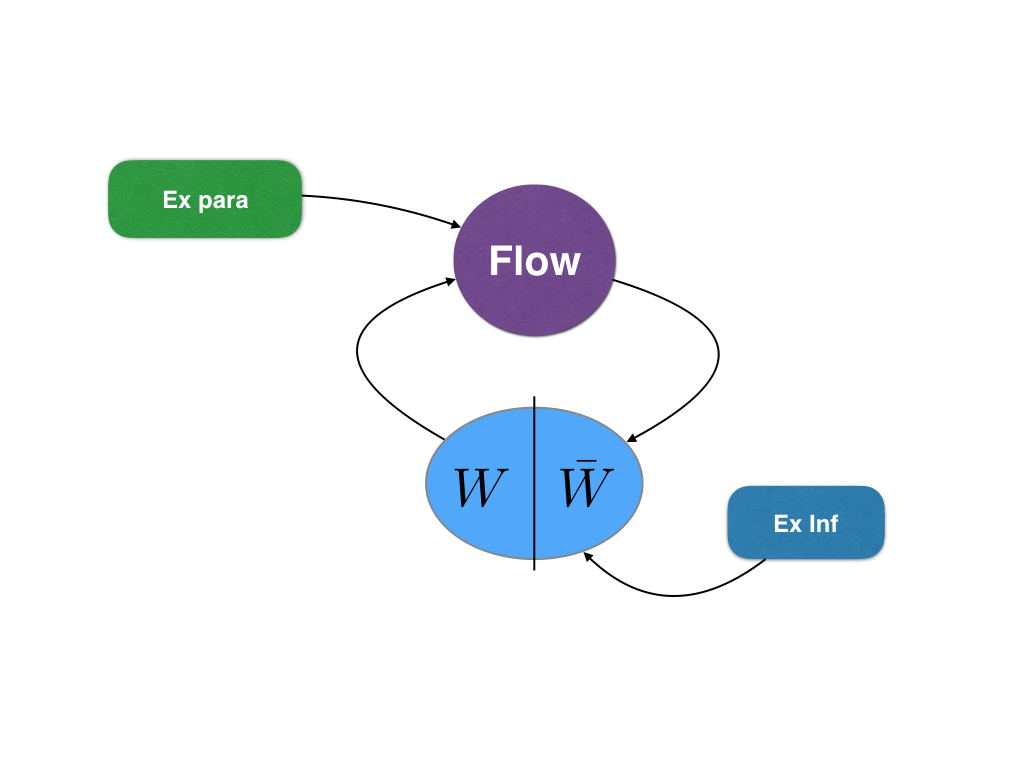
\includegraphics[width = 9cm]{picture/struc.jpg}
    %\end{center}
    \end{wrapfigure}
    Our model's structure is pretty clear.
    We using some prominent external parameters as the input of our dynamic system. To determine the water supply ability of a region, the most important part is the water flow which means the total amount of industrial, agricultural and residential consumption. The season we can use the consumption to measure the supply it that they must be the same during a long period just like the electricity use equal to the electricity produce.

    $$
    \langle \text{Consumption}\rangle = \langle \text{Supply} \rangle
    $$

    The $W$ and $\bar{W}$ is a crucial conception in our dynamic part, $W$ stand for the total clean water resource over a period, while the $\bar{W}$ is the total wasted water resource which can be transfered into $W$ after several processing steps.

  \subsection{Model Prominent Parameters}

    The prominent parameters are some thing the dynamics part heavily rely on, to find the prominent parameters, we need to investigate the relation between some alternative parameters and consumptions according to the past data. In other words, prominent parameters are not given before a specific research object is given, we just give some alternative parameters and using the past data to determine which is better related and which is less related to our dynamic part variables.

    Generally, there are several important alternative parameters like: Population, GDP Per Capita are of course important statistic numbers. Moreover, Agricultural Irrigation Area play an important role in agricultural consumption, Iron and Steel Production is also important in industrial consumption, and Engel's coefficient is an important statistical number about residential living which make it important in residential consumption.

  \subsection{Model Dynamics}

    The dynamics part of our model is inspired by the water cycle(Figure \ref{water cycle})\cite{WaterCycle}
    \begin{figure}[!hb]
    \begin{center}
    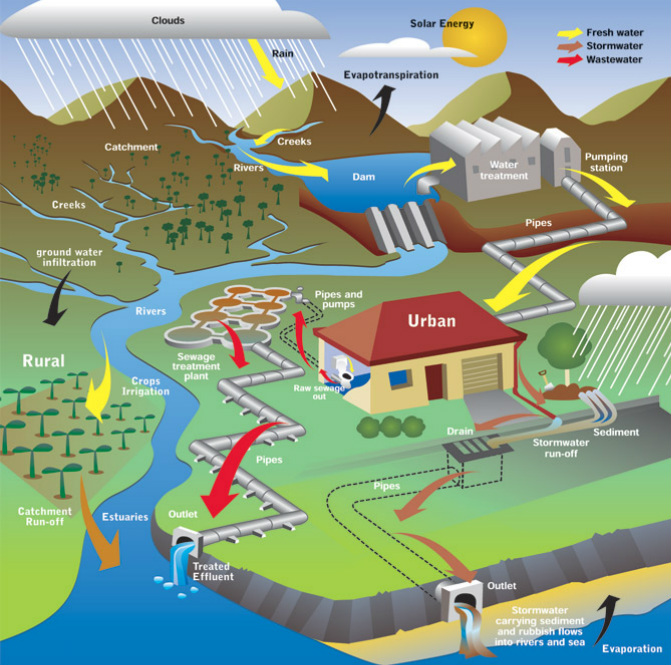
\includegraphics[width = 10cm]{picture/UrbanWaterCycle.jpg}
    \caption{water cycle}
    \label{water cycle}
    \end{center}
    \end{figure}


  \subsection{How to apply our model}

    With good structure of our model and program, the application of our model can be done in a pretty clear way.

    \begin{enumerate}[step 1]
      \item Using the data of alternative prominent parameters and consumption variables in the past to find the strength of correlation, Spearman or Pearson or other coefficients.
      \item According to the analysis of step 1, we can  determine the specific evolution equations of consumption variables which depend on the prominent parameters and water resource $W$ and $\bar{W}$.
      \item Using the past data of needed prominent parameters, we will be able to use fitness method to predict the future data of prominent parameters as the input of evolution equations.
      \item Using the Iterative method, we can predict the variables in dynamics part thus we can get the Output -- the water supply per person (A) to judge the water situation in a specific future time of a certain region.
    \end{enumerate}

\section{China's water scarcity}
  According to the UN water scarcity map\cite{WaterScarcityMap}, China is a country with water stress,
  \begin{wrapfigure}{l}{7cm}
  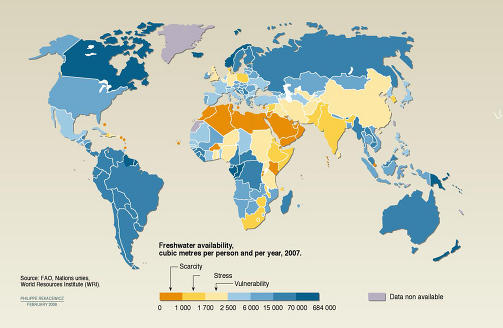
\includegraphics[width = 6cm]{picture/WaterScarcityMap.jpg}
  \end{wrapfigure}
  which make it a region where water is moderately overloaded. In our consideration, level 2, will provide more abundant behavior in a dynamical model(will it become water scarce or water sufficient in the future?). Thus we pick up China as our research object. To make our model more predictable and more reality connected. We will continue our investigation with the data from National Bureau of Statistics of the People's Republic China\cite{ChinaDataBase}.
  According to our models, the following variables are prominent: the Population, the GDP, the water consumption and the total water resource.
  We grab all the data and try to analyses them and they relation.

  \subsection{Prominent variables' tendency}
  Using proper assumption and the past data in databases. We can using fitness method to determine the time dependency of our alternative parameters.
  In our consideration, following factors especially eye-catching.
  \begin{table}[!h]
  \begin{tabular}{|c|c|}
  \hline
  $P$ & Population \\
  \hline
  $\text{PCGDP}$ & Per Capita Gross Domestic Product \\
  \hline
  $\text{IA}$ & Irrigation Area \\
  \hline
  $\text{ISP}$ & Iron and Steel Production \\
  \hline
  $\text{ElP}$ & Electricity Production. \\
  \hline
  $\text{EnC}$ & Engel's Coefficient \\
  \hline
  \end{tabular}
  \end{table}
  For further convenience, we will investigate their relation towards time at first.
    \subsubsection{Population}
      The population growth model is various, for best concern, we use Logistic Model as the Population evolution model thus we can use the solution--Standard logistic sigmoid function as our target function by adding three basic coefficients.
      $$
      P(t) = \frac{K_p}{1+\exp[-\lambda_p(t-t_0)]}
      $$
      {\huge figure}
    \subsubsection{Per Capita Gross Domestic Product}
      As the largest developing country over the world, China has pretty high PCGDP growth rate. It seems like an exponential growth However, according to our data browse, some developed countries have already reach some obstacles. Thus we think it will be suitable if we apply Logistic model in the fitness model of $\text{PCGDP}$.
      $$
      \text{PCGDP}(t) = \frac{K_\text{PCGDP}}{1+\exp[-\lambda_\text{PCGDP}(t-t_0)]}
      $$
      {\huge figure}
    \subsubsection{Irrigation Area}

    {\huge figure}
    \subsubsection{Iron and Steel Production}

    {\huge figure}
    \subsubsection{Electricity Production}

    {\huge figure}
    \subsubsection{Engel's Coefficient}
    $$
    \begin{cases}
    \text{Enc}_{urban}(t) = \frac{C_{urban}}{t-t_0} \\
    \text{Enc}_{rural}(t) = \frac{C_{urban}}{t-t_0}
    \end{cases}
    $$

  \subsection{Relation between prominent parameters and variables}
    To investigate the relation between prominent parameters and variables, we firstly introduce the conception of  correlation. In statistics, dependence is any statistical relationship between two random variables or two sets of data, and correlation refers to any of a broad class of statistical relationships involving dependence.


    \paragraph{Pearson product-moment correlation coefficient} is a measure of the linear correlation between two variables $X, Y$. If there is two datasets $\{x_1,x_2,\ddots, x_n\}$ and $\{y_1,y_2,\ddots, y_n\}$, then the formula for r is:
    $$
    r = \frac{\sum{(x_i-\bar{x})(y_i-\bar{y})}}{\sqrt{\sum{(x_i-\bar{x})^2}}\sqrt{\sum{(y_i-\bar{y})^2}}}
    $$

    \paragraph{Spearman's rank correlation coefficient} is a nonparametric measure of statistical dependence between two variables. It assesses how well the relationship between two variables can be described using a monotonic function. If there are no repeated data values, a perfect Spearman correlation of $+1$ or $-1$ occurs when each of the variables is a perfect monotone function of the other\cite{Spearman}\cite{spearmanr}. The Spearman correlation coefficient is defined as the Pearson correlation coefficient between the ranked variables\cite{ranked variable}. For a sample of size n, the n raw scores $X_i,Y_i$ are converted ranks $x_i, y_i$, and $\rho$ is computed from:
    $$
    \rho = 1 - \frac{6\sum{(x_i-y_i)^2}}{n(n^2-1)}
    $$

    \paragraph{Kendall rank correlation coefficient} is a statistic used to measure the association between two measured quantities. Let $(x_1, y_1),(x_2, y_2),\ddots,(x_n, y_n)$ be a set of observations of the joint random variables X and Y respectively, such that all the values of $(x_i)$ and $(y_i)$ are unique. Any pair of observations $(x_i,y_i)$ and $(x_j, y_j)$, where $i\neq j$, are said to be concordant if the ranks for both elements agree: that is, if both $x_i > x_j$ and $y_i > y_j$ or if both $x_i < x_j$ and $y_i < y_j$. They are said to be discordant, if $x_i > x_j$ and $y_i < y_j$ or if $x_i < x_j$ and $y_i > y_j$. If $x_i = x_j$ or $y_i = y_j$, the pair is neither concordant nor discordant. Thus the $\tau$ coefficient is defined as\cite{Kendall}\cite{kendalltau}:
    $$
    \tau = \frac{(\text{number of concordant pairs}) - (\text{number of discordant pairs})}{1/2 n (n-1)}
    $$

    Using coefficients above, we get a map about the relation between prominent parameters and consumption variables.

    {\huge Coefficients Table}

  \subsection{Fitness of past data using dynamic model}


\section{Prediction of water situation}
  In our model external variables are used for future prediction.


\section{Intervention plan designing}

\section{Prediction with Intervention plan}

\section{Conclusion}


\begin{thebibliography}{99}
  \bibitem{AbilityMeasure} {Falkenmark and Lindh 1976, quoted in UNEP/WMO.Climate Change 2001: Working Group II: Impacts,Adaptation and Vulnerability. UNEP. Retrieved 3 February 2009.}
  \bibitem{WaterScarcityMap} http://www.unep.org/dewa/vitalwater
  \bibitem{WaterCycle} trinityrivertexas.org, Living with the Trinity Lesson Plan 1: The Natural Water Cycle and the Urban Water Cycle
  \bibitem{ChinaDataBase} http://www.stats.gov.cn
  \bibitem{Spearman} https://en.wikipedia.org/wiki/Spearman\%27s\_rank\_correlation\_coefficient
  \bibitem{spearmanr} Zwillinger, D. and Kokoska, S. (2000). CRC Standard Probability and Statistics Tables and Formulae. Chapman \& Hall: New York. 2000. Section 14.7
  \bibitem{ranked variables} Myers, Jerome L.; Well, Arnold D. (2003). Research Design and Statistical Analysis (2nd ed.). Lawrence Erlbaum. p. 508
  \bibitem{Kendall} https://en.wikipedia.org/wiki/Kendall\_rank\_correlation\_coefficient
  \bibitem{kendalltau} W.R. Knight, “A Computer Method for Calculating Kendall’s Tau with Ungrouped Data”, Journal of the American Statistical Association, Vol. 61, No. 314, Part 1, pp. 436-439, 1966

\end{thebibliography}


%==========================================================

\begin{comment}
%===============================appendices===============================
    \begin{appendices}
    %\renewcommand{\thesection}{\Alph{chapter}.}

      \section{First appendix}

    some text...


Here are simulation programmes we used in our model as follow.\\


\textbf{\textcolor[rgb]{0.98,0.00,0.00}{Input matlab source:}}
\lstinputlisting[language=Matlab]{./code/matlab1.m}


      \section{Second appendix}

    some more text\textcolor[rgb]{0.98,0.00,0.00}{\textbf{Input C++ source:}}
\lstinputlisting[language=C++]{./code/sudoku.cpp}

    \end{appendices}

\end{comment}